%BAB_3 LAPORAN KP

\chapter{PERANCANGAN SISTEM}

\section{Metode Perancangan sistem}
Perancangan robot serpent-2 ini diawali dengan menentukan metode yang tepat untuk mendesain dan membangun sistem secara keseluruhan meliputi perancangan elektronis,pemrograman pada Arduino Mega 2560, implementasi kinematika robot pada robot serpent-2, serta perancangan antarmuka pada \emph {processing ide}.Metode perancangan sistem meliputi diagram blok, flowchart cara kerja sistem, prinsip kerja dan perancangan tiap segmen-segmen yang dibutuhkan.
	
	\subsection{Diagram Blok Perancangan Sistem}
	Pada dasarnya, perancangan sistem untuk robot serphent-2 secara sederhana dapat dibagi menjadi tiga bagian. Ketiga perancangan ini merupakan hal yang sangat penting dan saling berkaitan.Perancangan robot serphent=2 jika digambarkan dalam diagram blok sistem dapat digambarkan seperti yang ditunjukkan dalam gambar 3.1
	\begin{figure}[H]
		\centering
		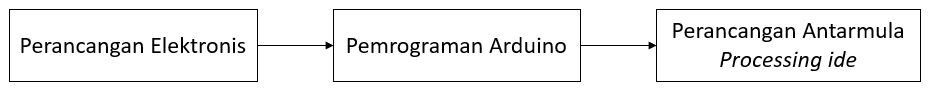
\includegraphics[width=\linewidth]{gambar/diagram_blok.jpg}
		\caption{Diagram metode perancangan sistem.}
	\end{figure}

\subsection{Flowchart Cara Kerja Sistem}
Kerja sistem, merupakan bagaimana robot serphent-2 melakukan tugasnya sesuai perintah yang dimasukkan dan kemudian dilaksanakan oleh aktuator.Robot serphent-2 memiliki kerja sistem yang tergolong ringkas yang mana didominasi oleh sistem maju tetapi juga memiliki sistem balik.  Kerja sistem dari robor serphent 2 jika dirancang dalam bentuk flowchat dapat ditunjukkan seperti dalam gambar 3.2

\begin{figure}[H]
	\centering
	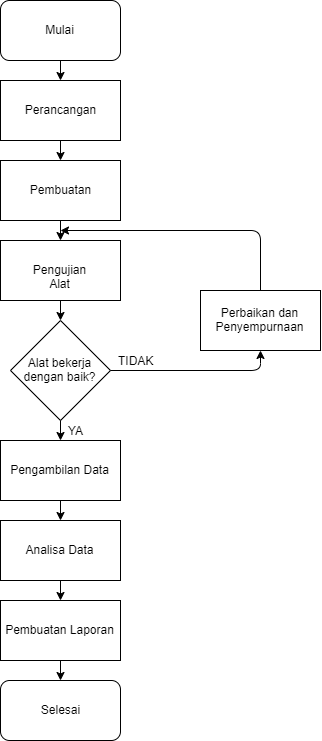
\includegraphics[width=8cm	]{gambar/flowchart.png}
	\caption{Flowchat cara kerja sistem.}
\end{figure}
	
	\subsection{Perancangan Elektronis}
	Perancangan elektronis merupakan perancangan dasar pada pembuatan suatu sistem. Suatu sistem dapat bekerja secara maksimal karena terdiri dari komponen-komponen yang memiliki fungsi masing-masing. Komponen-komponen ini, disatukan kedalam sebuah \textit{Shield} \textit{Printed Circuit Board} (PCB). 
	
	\begin{enumerate}
		\item Pengendali motor DC yang digunakan adalah modul EMS 30A H-Bridge sebanyak tiga buah yang masing-masing untuk menggerakkan \textit{Shoulder, Elbow} dan perputaran \textit{Wrist}. Secara garis besar, fungsi modul pengendali motor ini adalah untuk mengendalikan arah dan kecepatan putaran motor DC sesuai instruksi kendali dari Arduino Mega 2560 pengguna.Modul akan menerima nilai yanf dikirimkan oleh Arduino Mega 2560 dan kemudian menggerakan motor servo yang sudah terhubung dengan \textit{shoulder, Elbow} dan perputaran dari \textit{Wirst}.
		
		\begin{figure}[H]
			\centering
			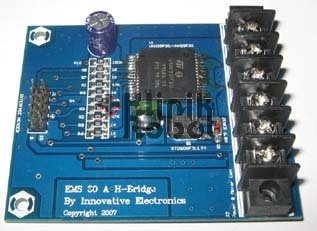
\includegraphics[width=5cm	]{gambar/driver_motor.jpg}
			\caption{Pengendali Motor DC EMS 30A H-Bridge}
		\end{figure}
		
		\item Potensiometer yang digunakan adalah jenis potensiometer \textit{rotary}. Potensiometer ini sebagai sensor posisi motor servo. Potensiometer terpasang pada setiap bagian motor servo sesuai dengan perputarannya dan akan memberikan keluaran berupa level tegangan yang berubah-ubah sesuai dengan posisi motor servo saat itu. Level tegangan tersebut kemudian dikirimkan kepada Arduino Mega 2560 sebagai sensor \textit{feedback} yang nantinya akan diproses untuk menyempurnakan posisi sesuai yang ditentukan.
		\begin{figure}[H]
			\centering
		%	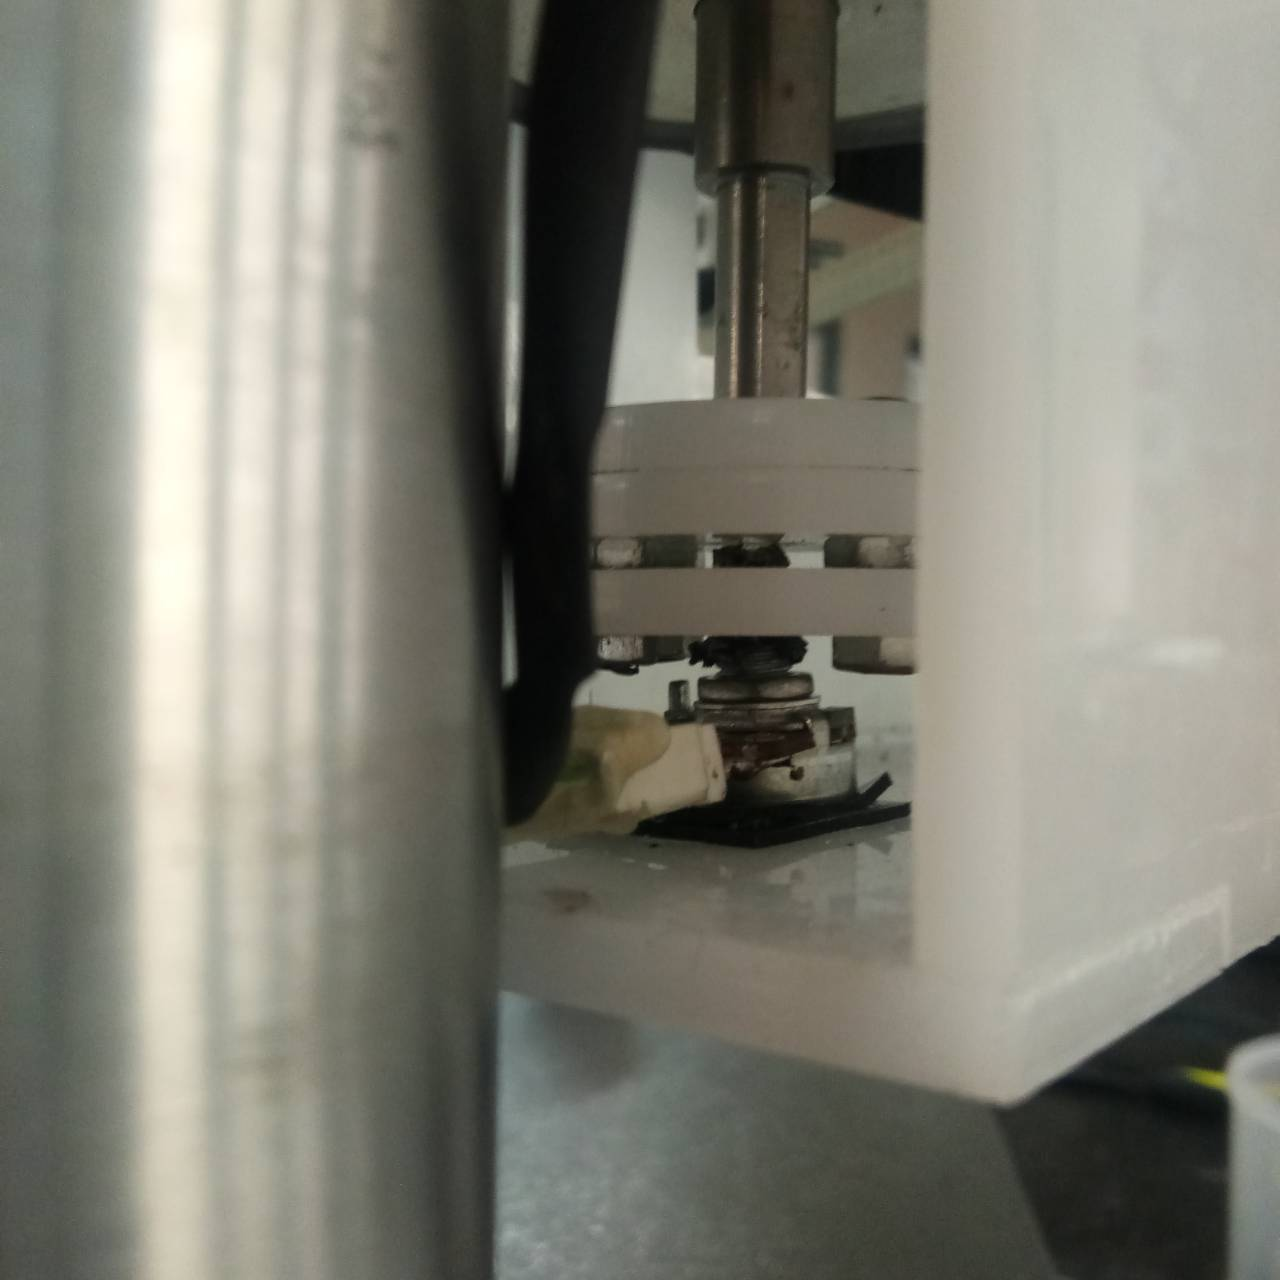
\includegraphics[width=5cm	]{potensio.jpg}
			\caption{Mekanisme pemasangan potensiometer pada motor}
		\end{figure}
		
		\item Pengaturan pergerakan vertikal dari \textit{wirst} pada robot serphent-2 menggunakan sistem pneumatik silinder. Pada bagian buka tutup \textit{wirst} menggunakan masukan udara biasa untuk menutupnya dan membuang udara unutk membukanya. Udara tersebut didapat dari kompresor yang terhubung melalui selang dan dikontrol melalui sebuah relay yang bekerja pada tegangan 24v.
		
		\begin{figure}[H]
			\centering
		%	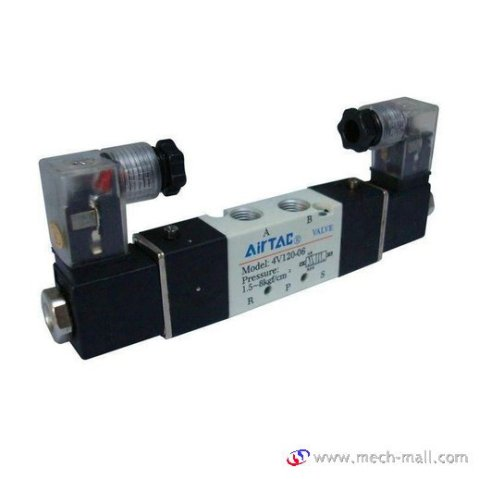
\includegraphics[width=5cm	]{relay.jpg}
			\caption{Relay pneumatik}
		\end{figure}
		\begin{figure}[H]
			\centering
		%	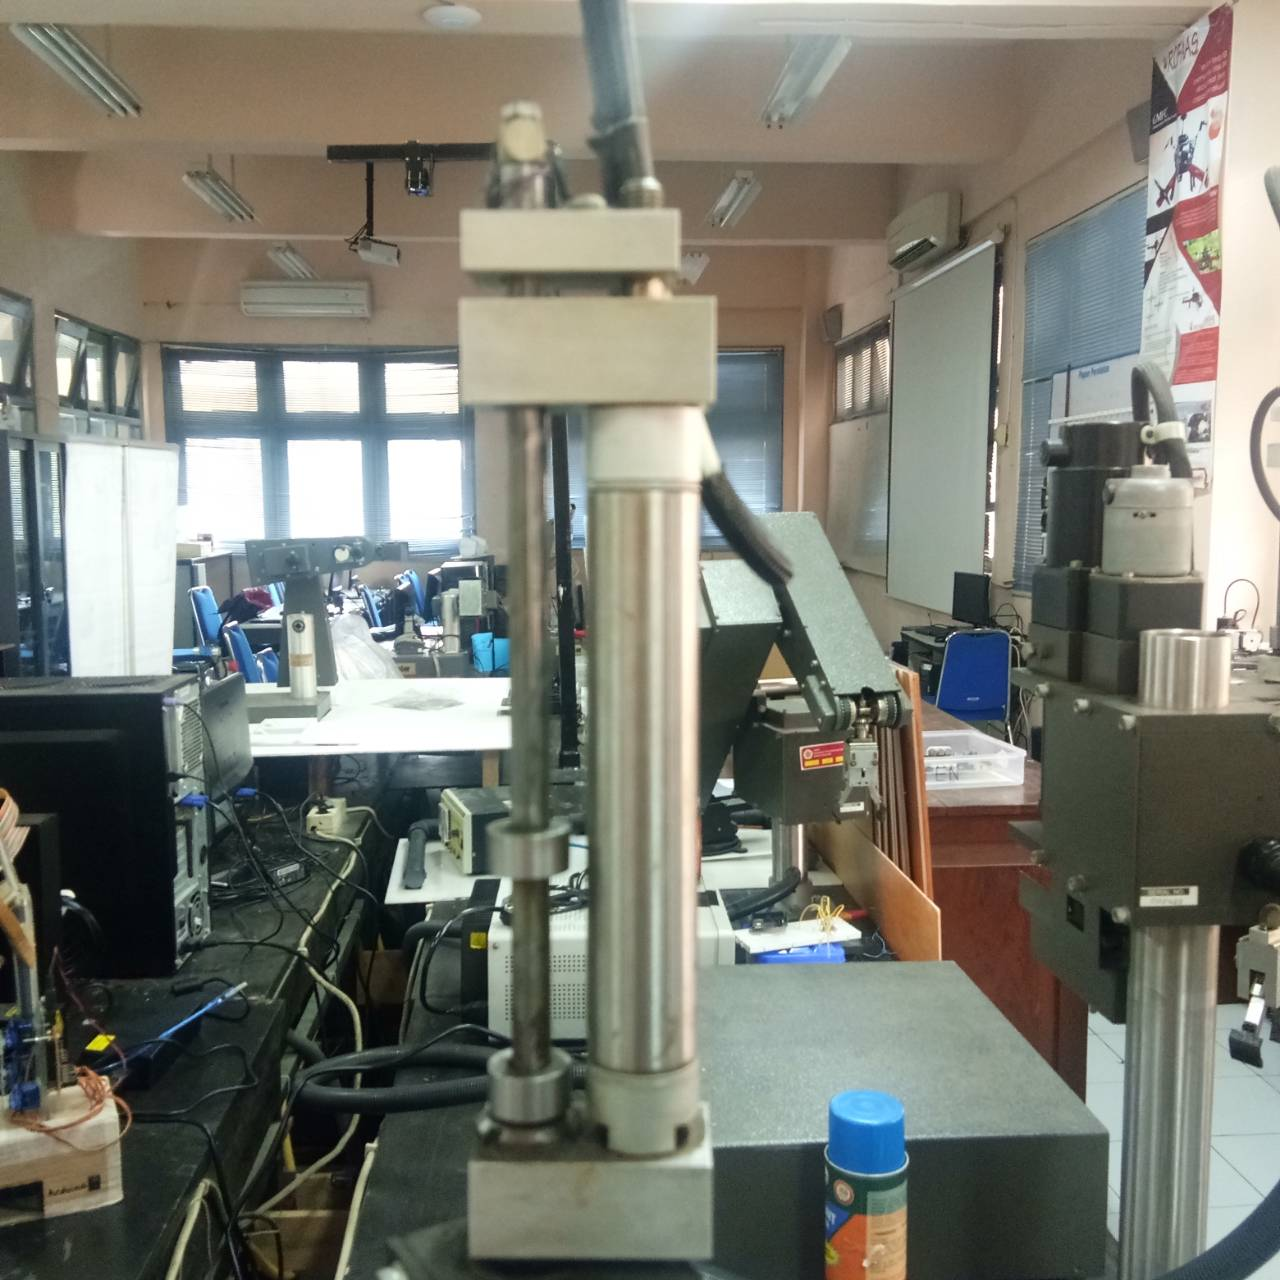
\includegraphics[width=5cm	]{relay2.jpg}
			\caption{Pneumatik Silinder}
		\end{figure}
		
		\item Relay yang bekerja pada tegangan 24v, pada Arduino Mega 2560 dikontrol melalui sinyal digital dengan bantuan rangkaian yang menggunakan TIP31A yang berfungsi untuk memutus atau membuka tegangan 24v. 
		\begin{figure}[H]
			\centering
		%	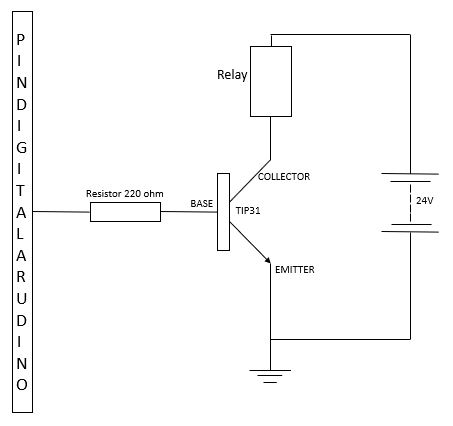
\includegraphics[width=5cm	]{relay3.jpg}
			\caption{Rangkaian skematik TIP31 sebagai \textit{switch}}
		\end{figure}
		
		\item Semua komponen-komponen yang dibutuhkan pada sistem kerja, disatukan ke dalam \textit{shield PCB} yang bertujuan agar meringkaskan serta memudahkan perangkaian elektronis. Rangkaian PCB dibuat melalui \textit{software} Eagle.
		\begin{figure}[H]
			\centering
		%	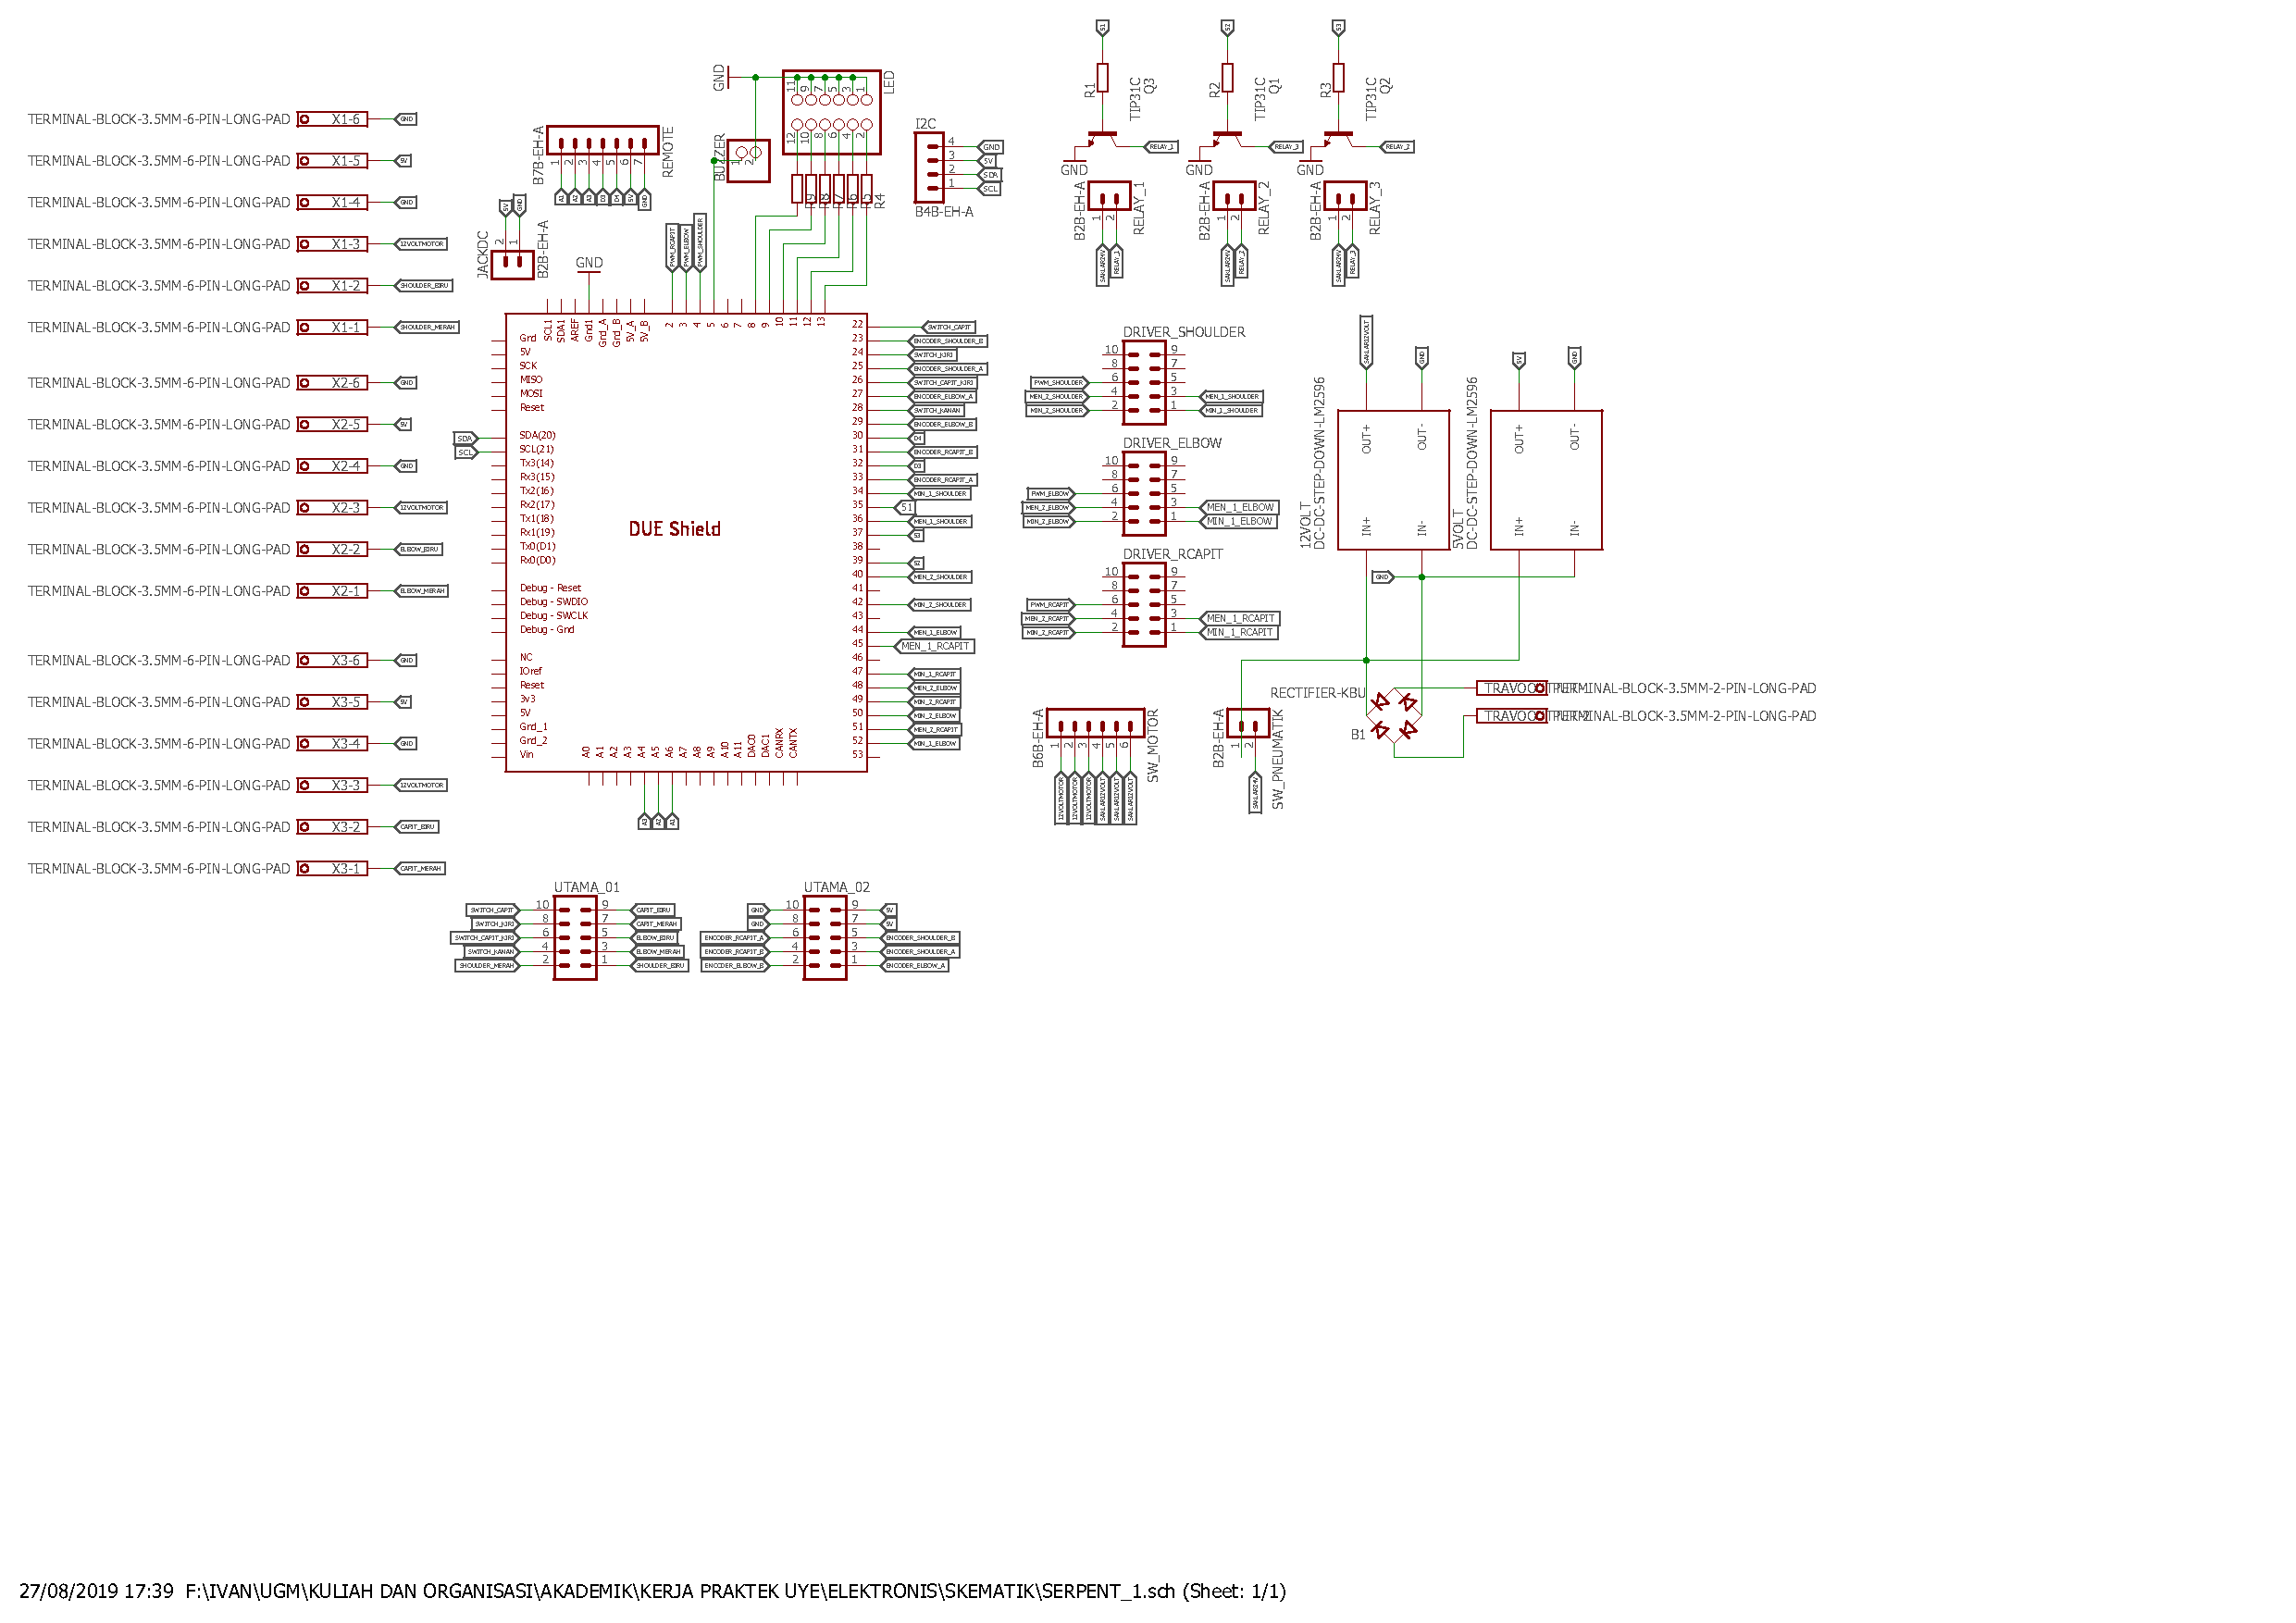
\includegraphics[width=15cm	]{skematik.pdf}
			\caption{Skematik rangkaian elektronis keseluruhan}
		\end{figure}
		
		
	\end{enumerate}
	\subsection{Perancangan Elektronis}
	
	\subsection{Pemrograman Kontroller \& Implementasi PID}
	
	\subsection{Perancangan Antar Muka \& Inplementasi \textit{Invers Kinematic}}
	